%!TEX root=bare_conf.tex
\section{Problem Description}\label{sec:description}
The targeted problem in this paper is the dynamic memory leaks - A block of heap memory space is being leaked if the program or the run-time system does not reclaim its memory when the lifetime of heap memory space has ended. 
The lifetime of heap memory space is represented in three ways in existing works~\cite{OR06}: 
\begin{itemize}
\item
\textit{Referencing:} the lifetime of a block of a heap memory space ends when there are no references to the space (excluding references from abandoned spaces).
\item 
\textit{Reachability:} the lifetime of a heap memory space ends when it is no longer reachable from program variables.
\item 
\textit{Liveness:} the lifetime of a heap memory space ends after the last access to that space.
\end{itemize}
This paper focuses on the second view - reachability, as reasoning on the reachability is more intuitive in the CFG, and our analysis is based on it.
In the reachability view, there is a memory leak if the lifetime of a heap memory space ends while the memory pointer can not reach to that space.
%This paper analyzes the reasons for memory leaks from the perspective of control flow, which is based on the second way - reachability. 
Since our approach is based on CFG, detecting memory leaks is essentially analyzing whether the memory pointers have been freed when the lifetime of the corresponding memory spaces end in each branch of the control flow graph. Therefore, the memory detection can be converted into a control flow graph analysis on the correspondence relation between the memory pointers and the lifetime of the corresponding memory spaces, referred to as the reachability of the pointers.

As stated in Section~\ref{sec:intro}, when procedure $P$ has multiple control flow branches, the pointers pointing to corresponding memory spaces may be freed in wrong order, and the allocation and deallocation of memory space may appear in different control flow branches, this increases the complexity of the control flow graph analysis, because of the complex branch guarding condition analysis. %In addition, high control flow complexity will result in more difficult paths analysis. 
%The following definition defines the complex control flow.
This paper formally defines the complex control flow as follows.

\begin{definition}[Complex Control Flow]
Given that a directed graph named $G= (N, E)$ is the control flow graph of a procedure $P$, where $N$ denotes the set of nodes and $E$ denotes the set of edges, the control flow is called \emph{complex control flow} when the cyclomatic complexity of $G$, denoted as $V(G)$, is no less than $2$. That is $V(G)=D+1\geq 2$, where $D$ denotes the number of conditional and loop branching nodes.
\end{definition} 

Fig.~\ref{fig:1} displays this generation of complex control flow. A simple control flow graph of procedure $P$ with memory allocation and deallocation is shown on the left. After adding the control flow branches, a complex control flow graph is shown on the right. Therefore, detection system needs to analyze whether the memory spaces are released in each branch after being allocated. It should be noted that this section only considers the cases that allocate or release memory space of the same pointer, and the case that memory spaces are not fully released does not exist. There are four cases corresponding to the values of the two branches in the complex control flow graph:
\begin{enumerate}
\item
B1 =$\mathit{false}$, B2 = $\mathit{false}$: Corresponding to path 1-6-7. No memory leaks occur in this case, since there is no memory operations.
\item
B1 =$\mathit{true}$, B2 = $\mathit{false}$: Corresponding to path 1-2-3-7. The memory blocks have not been freed after being allocated, which is a typical kind of memory leaks.
\item 
B1 = $\mathit{false}$, B2 = $\mathit{true}$: Corresponding to path 6-4-5. The unallocated memory blocks are freed.
\item
B1 = $\mathit{true}$, B2 = $\mathit{true}$: Corresponding to path 1-2-3-4-5. Whether there is memory leak in this case is uncertain. The result relies on the number of executions of the memory allocation or deallocation related statements. Specifically, if both B1 and B2 are conditional branches, the memory allocation and deallocation will be executed only once, then there are no memory leaks in this structure. If B1 or B2 is a loop node, then the memory allocation or deallocation for the same pointer $p$ will be executed more than once in the loop, which will lead to a memory leak e.g., if B1 is a loop node, then multiple memory spaces are allocated, each in a single execution of the loop; but B2 is a conditional node, and thus there is only one deallocation in the branch. %In summary, the case that B1 =$\mathit{true}$ \&\& B2 =$\mathit{true}$ can be judged as memory leaks for the uncertainty of memory allocation and deallocation in static analysis.
\end{enumerate}

\begin{figure}[!h]
\center
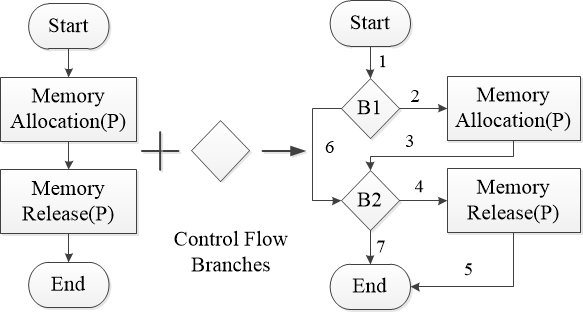
\includegraphics[width=0.45\textwidth]{figure/fig1-fig4/fig1}
\caption{Description of memory leaks reasons}
\label{fig:1}
\end{figure}

\begin{figure}[!h]
\center
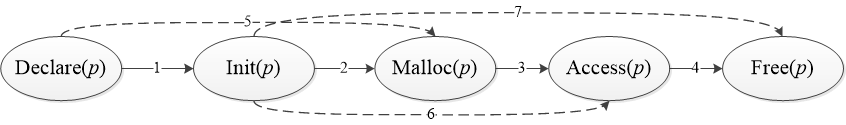
\includegraphics[width=0.45\textwidth]{figure/fig1-fig4/fig2}
\caption{Lifetime of a pointer $p$}
\label{fig:2}
\end{figure}

In each branch of the control flow graph, in addition to considering the allocation and deallocation of memory spaces, detection system needs to additionally consider the lifetime of each pointer, as shown in the definition of dynamic memory leaks. To provide some clue, Fig.~\ref{fig:2} shows the lifetime of a pointer $p$ pointing to a heap memory space, using C language as an example. This figure shows the lifetime of a pointer $p$ from being declared to being freed. The solid arrows represent the correct order. The dotted arrows represent all the cases that may result in the memory leaks on the memory blocks refereed by a single pointer $p$. In details, the dotted arrow $5$ shows the case that the pointer $p$ is not initialized before being allocated to memory blocks, arrow $6$ illustrates that the pointer $p$ is not allocated to memory blocks before being accessed, arrow $7$ presents that $p$ is not allocated to memory blocks before being freed.

Note that Fig.~\ref{fig:2} only shows the lifetime of one pointer. When multiple pointers are considered, the cases that may lead to memory issues are complicated, which is another challenge in the memory leak detection.
